\documentclass{article}
\usepackage{graphicx}
\usepackage{ragged2e}
\usepackage{amsmath}
\usepackage{makecell}
\usepackage{booktabs}

\title{Adaptive Temporal Horizons \\ in Auto-Regressive Models}
\author{Lena Fiedor}
\date{December 2026}

\begin{document}
\justifying
\maketitle

\section{Abstract}

Forecasting chaotic dynamical systems is challenging because small differences in initial conditions can grow rapidly, limiting the reliability of long-term predictions. In neural trajectory forecasting, the prediction horizon is therefore a central design choice: short horizons may lead to accurate but limited predictions, while long horizons can produce targets dominated by divergence and accumulated error. Most forecasting sets-ups use fixed prediction horizons, even though the predictability of chaotic trajectories may vary across different regions of the state space.

We investigate the adaptive temporal horizon for neural forecasting of chaotic dynamical systems. Instead of training only with a fixed prediction time, we let the horizon vary during training:
\begin{enumerate}
    \item Using a simple linear scheduler,
    \item Performing an online cross-validation,
    \item Mapping from the local predictability properties of the trajectory,
\end{enumerate}
The method is evaluated on benchmark chaotic systems, including the Lorenz63, Lorenz96 and Rössler systems, and compared against fixed-horizon baselines using the same amount of computational resources, accordingly. The evaluation considers the prediction accuracy for a fixed horizon $T = 1$ and analyzes whether adaptive horizon selection provides a more suitable training signal for chaotic trajectory forecasting.

Our results show that the horizon choice has a significant effect on forecasting performance and that adaptive temporal horizons can provide useful insight into the varying predictability of chaotic systems. Overall, we demonstrate that treating the prediction horizon as an adaptive component, rather than a fixed experimental parameter, is a promising direction for improving neural forecasting in chaotic dynamical systems.

\newpage

\tableofcontents
\newpage

\section{Introduction}

\subsection{Motivation}

Many systems in science and engineering evolve according to deterministic laws, yet their long-term behavior can be extremely difficult to predict. Chaotic dynamical systems are a central example of this tension: even when the governing equations are known, small differences in initial conditions can grow rapidly and lead to diverging trajectories. This makes forecasting such systems a useful test case for studying the limits of data-driven prediction.

In trajectory forecasting, the difficulty of the prediction strongly depends on the temporal horizon. Short-term predictions may remain close to the true trajectory, whereas longer-term predictions accumulate errors and eventually become unreliable \cite{aceituno_temporal_2025}. When finding an optimal fixed prediction horizon, one needs some ground truth about the model, as it depends on the local dynamics of the system as well as model parameters, e.g. chosen timestep. The fixed horizon may also not reflect how predictability varies across different regions of the state space.

This paper investigates the adaptive temporal horizon as a solution to the performance-learnability trade-off \cite{aceituno_temporal_2025}. We argue that instead of performing a computationally expensive grid search for an optimal fixed temporal horizon parameter, this process can be automatized by training the model with variable horizon and taking into account the local predictability of the system.

\subsection{Problem Statement}

A common approach in data-driven trajectory forecasting is to train and evaluate models at a fixed prediction horizon. Although this approach provides a clear and comparable learning objective, it also assumes that the arbitrarily chosen horizon parameter is able to capture well the local dynamics; moreover, it assumes that the same temporal distance is equally appropriate throughout the trajectory. This assumption is restrictive for chaotic dynamical systems, where local rates of divergence can vary substantially over the state space, They may also not be of monotonic nature, meaning that chosen horizon parameter $k$ does not capture well the behavior of errors of some other periodicity, for example $\frac{k+1}{2}$ \cite{zhuang_horizon_2025}. As a result, some regions may remain predictable over relatively long horizons, while others may become unreliable much sooner.

Finding an optimal prediction horizon is a computationally demanding task. Treating the horizon optimization problem as a function of computational resources, we propose replacing the grid search for the horizon parameter with one adaptive model.

Furthermore, we raise the question of whether adapting the prediction horizon to the local dynamics of the system can provide a suitable training signal for neural forecasting models. We extend our model by mapping the trajectory uncertainty measured by Local Lyapunov Exponents (LLEs) to the temporal horizon.

\subsection{Aim and Research Questions}

We investigate whether adaptive temporal horizons can improve neural forecasting of chaotic dynamical systems compared with fixed-horizon training using the same amount of computational resources. Furthermore, we employ the local predictability score of the system to guide the horizon choice.

\subsection{Contributions}

The main contributions of this paper are as follows.

\begin{enumerate}
    \item A formulation of adaptive temporal horizon selection for neural forecasting of chaotic dynamical systems.
    \item An implementation of a training framework for four types of adaptive horizon neural forecasting models.
    \item An empirical evaluation on benchmark chaotic systems, including the Lorenz63, Lorenz96 and Rössler systems.
    \item Comparison of forecasting performance across horizons showing how adaptive horizon selection affects prediction accuracy and robustness compared to the fixed-horizon baseline.
\end{enumerate}

\newpage

\section{Background}

\subsection{Dynamical Systems and Chaotic Behavior}

Dynamical system is a description of how a system evolves over time. There exist two types of them: differential equations and iterated maps. The former describe system evolution in continuous time, while the latter arise in problems where time is discrete \cite{strogatz_nonlinear_1994}. This thesis focuses on differential equations.

The following formula provides a general framework for describing differential equations.

$$
\dot{x}(T) = f(x(t))
$$

Where the overdot denotes differentiation with respect to $t$.

We focus particularly on chaotic systems, a subset of dynamical systems that exhibits extreme sensitivity to initial conditions and can be characterized by its chaotic attractor, meaning a set of points towards which the system evolves \cite{aceituno_temporal_2025}.

One clarification that must be provided concerns the concept of time in the simulations. In order to approximate dynamical systems with neural networks, one needs to discretize the time step. In this paper, separate symbols are used to denote different time concepts.

\begin{itemize}
    \item $\tau$: Physical time,
    \item $dt$: Timestep used in the simulation,
    \item $T$: Discrete time horizon.
\end{itemize}

The relationship between these terms gives $\tau = dt \cdot T$.

\subsection{Benchmark Dynamical Systems} \label{dynamical_systems}

As a baseline, we selected two distinct three-dimensional chaotic systems: Lorenz63, Lorenz96, and Rössler attractors. Their dynamics have been extensively studied, allowing us to draw on previous work to obtain reliable ground-truth reference values \cite{ayers_supervised_2023}.

\paragraph{Lorenz63 attractor.} The Lorenz63 system (referred to simply as Lorenz), originally introduced as a simplified model of atmospheric convection, is defined as

\begin{equation}
    \dot{x}=\sigma(y-x), \qquad
    \dot{y}=x(\rho-z)-y, \qquad
    \dot{z}=xy-\beta z,
\end{equation}

With the standard parameter values $\sigma=10$, $\rho=28$, and $\beta=8/3$ \cite{lorenz_deterministic_1963}.

\paragraph{Rössler attractor.} The Rössler system was designed as a comparatively simple continuous-time model of chaos and is governed by

\begin{equation}
    \dot{x}=-y-z, \qquad
    \dot{y}=x+ay, \qquad
    \dot{z}=b+z(x-c)
\end{equation}

For which we use the commonly adopted chaotic parameter configuration $a=0.2$, $b=0.2$, and $c=5.7$ \cite{rossler_equation_1976}.

The system trajectories were obtained by numerically integrating the governing differential equations using the classical fourth-order Runge-Kutta method with a fixed time step ($\Delta t = 0.01$).

\paragraph{Lorenz96 attractor.} The Lorenz96 system is defined as follows. For $i = 1, ..., N$:

\begin{equation}
    \frac{dx_i}{dt} = (x_{i+1} - x_{i-2})x_{i-1} - x_i + F
\end{equation}

Where it is assumed that $x_{i-1} = x_{N-1}$, $x_0 = x_N$, $x_{N+1} = x_1$ and $N \geq 4$. We set the parameters of the system to $N = 10$ and $F = 8$ (the forcing constant).

\subsection{Global and Local Lyapunov Exponents}

\paragraph{Global Lyapunov Exponent.}
Chaotic systems exhibit behaviors that become unpredictable with time. To estimate the degree to which making such predictions is reliable, we use the Lyapunov exponents as a metric. By definition, they characterize the exponential divergence rate of two infinitesimally close trajectories.

To give an intuition, let us imagine a point in phase space that gets perturbed by an infinitesimally small vector $\delta_0$. The rate at which the original and perturbed trajectories separate from each other is described as follows.

\begin{equation}
    \vert \delta(t) \vert \approx e^{t \lambda} \vert \delta_0 \vert
\end{equation}

Here, $\lambda$ is the Lyapunov exponent. Since the perturbation vector can have different orientations for which the separation rate also varies, there exists a spectrum of Lyapunov exponents, equal in number to the dimensionality of the system. The largest $\lambda$, known as the maximal Lyapunov exponent (MLE), indicates that the system is chaotic \cite{noauthor_lyapunov_2026}.

Formally, we can define the maximal Lyapunov exponents as follows.

\begin{equation}
    \lambda = \lim_{t \rightarrow \infty} \lim_{\vert \delta_0 \vert \rightarrow 0} \frac{1}{t} \ln{\frac{\vert \delta(t) \vert}{\vert \delta_0 \vert}}
\end{equation}

\paragraph{Lyapunov Time.} The inverse of MLE, referred to as Lyapunov time, gives an estimate of rollout length for which predicting system's behavior is reliable. If $\lambda$ is positive, that is, the system exhibits chaotic behavior, the system cannot be predicted for more than a few multiples of $\frac{1}{\lambda}$ \cite{strogatz_nonlinear_1994}.

\paragraph{Local Lyapunov exponents.}
Although MLE is a useful metric, it does not tell anything about local predictability. Taking the Lorenz system as an example, one could imagine that trajectories in the phase space that start closer to the origin are harder to predict than those that start further away from the center, on the lobes of the butterfly-shaped graph (see Fig. \ref{fig:lorenz_lle_heatmap}). A small perturbation introduced in the central region can produce different subsequent lobe sequences when the trajectory either stays on the same side of the attractor or crosses the origin and switches to the other lobe. This variation is not represented by the global MLE, which summarizes the average expansion rate over the entire attractor.

In order to estimate local predictability around a given point on the trajectory, we introduce local Lyapunov exponents (LLE). Effectively, LLEs measure short-term perturbation growth in the neighborhood of individual trajectory states. A positive largest LLE indicates local expansion of nearby trajectories and therefore lower local predictability, whereas a negative value indicates local contraction and greater short-term predictability.

LLEs are calculated by evolving small perturbations alongside the system trajectory. At each time step, the perturbations are propagated using the Jacobian of the system and then orthonormalized by QR decomposition \cite{benettin_lyapunov_1980, dieci_lyapunov_2002}. The local exponents are obtained from the diagonal entries of the resulting upper-triangular matrix:

\begin{equation}
    \lambda^{loc}_{i, k} = \frac{1}{\Delta t} \log{\vert R_{ii, k} \vert}
\end{equation}

Where $\Delta t$ is the integration step. Positive values indicate local expansion of nearby trajectories, whereas negative values indicate local contraction.

\paragraph{Finite-time Lyapunov exponents.}
LLEs are not a good approximation for assigning a forecast horizon to an individual training sample for three reasons. First, they are one-step quantities: they measure stretching over a single interval $\Delta t$, are dominated by the local Jacobian, and fluctuate strongly along the attractor (they are frequently negative even in globally chaotic regions). Second, they are \emph{backward-looking}: the orthonormal frame $\mathbf{Q}_n$ carried along by the QR iteration has, after a transient, aligned with the backward Lyapunov vectors. The LLE at $\mathbf{x}_n$ therefore describes how a perturbation that has \emph{already} grown in the past is stretched at the current step, not how an arbitrary initial error at $\mathbf{x}_n$ will grow over the forecast window that starts there. Third, error growth over $T$ steps is governed by the \emph{product} of tangent maps. Because these maps are generally non-normal, the time-averaged LLEs do not, in general, give the maximal finite-horizon amplification, and transient growth is missed. These issues motivate the use of the forward \emph{finite-time Lyapunov exponent} (FTLE). The FTLE is anchored at the start state of each sample. It is computed over a window that matches the training horizon, and it measures the worst-case amplification of an initial perturbation over that window, independently of any inherited frame. As $T \to \infty$ it converges to the largest global Lyapunov exponent $\lambda_1$ for almost every initial condition, it interpolates between a purely local and a purely global description of predictability.

\begin{figure}
    \centering
    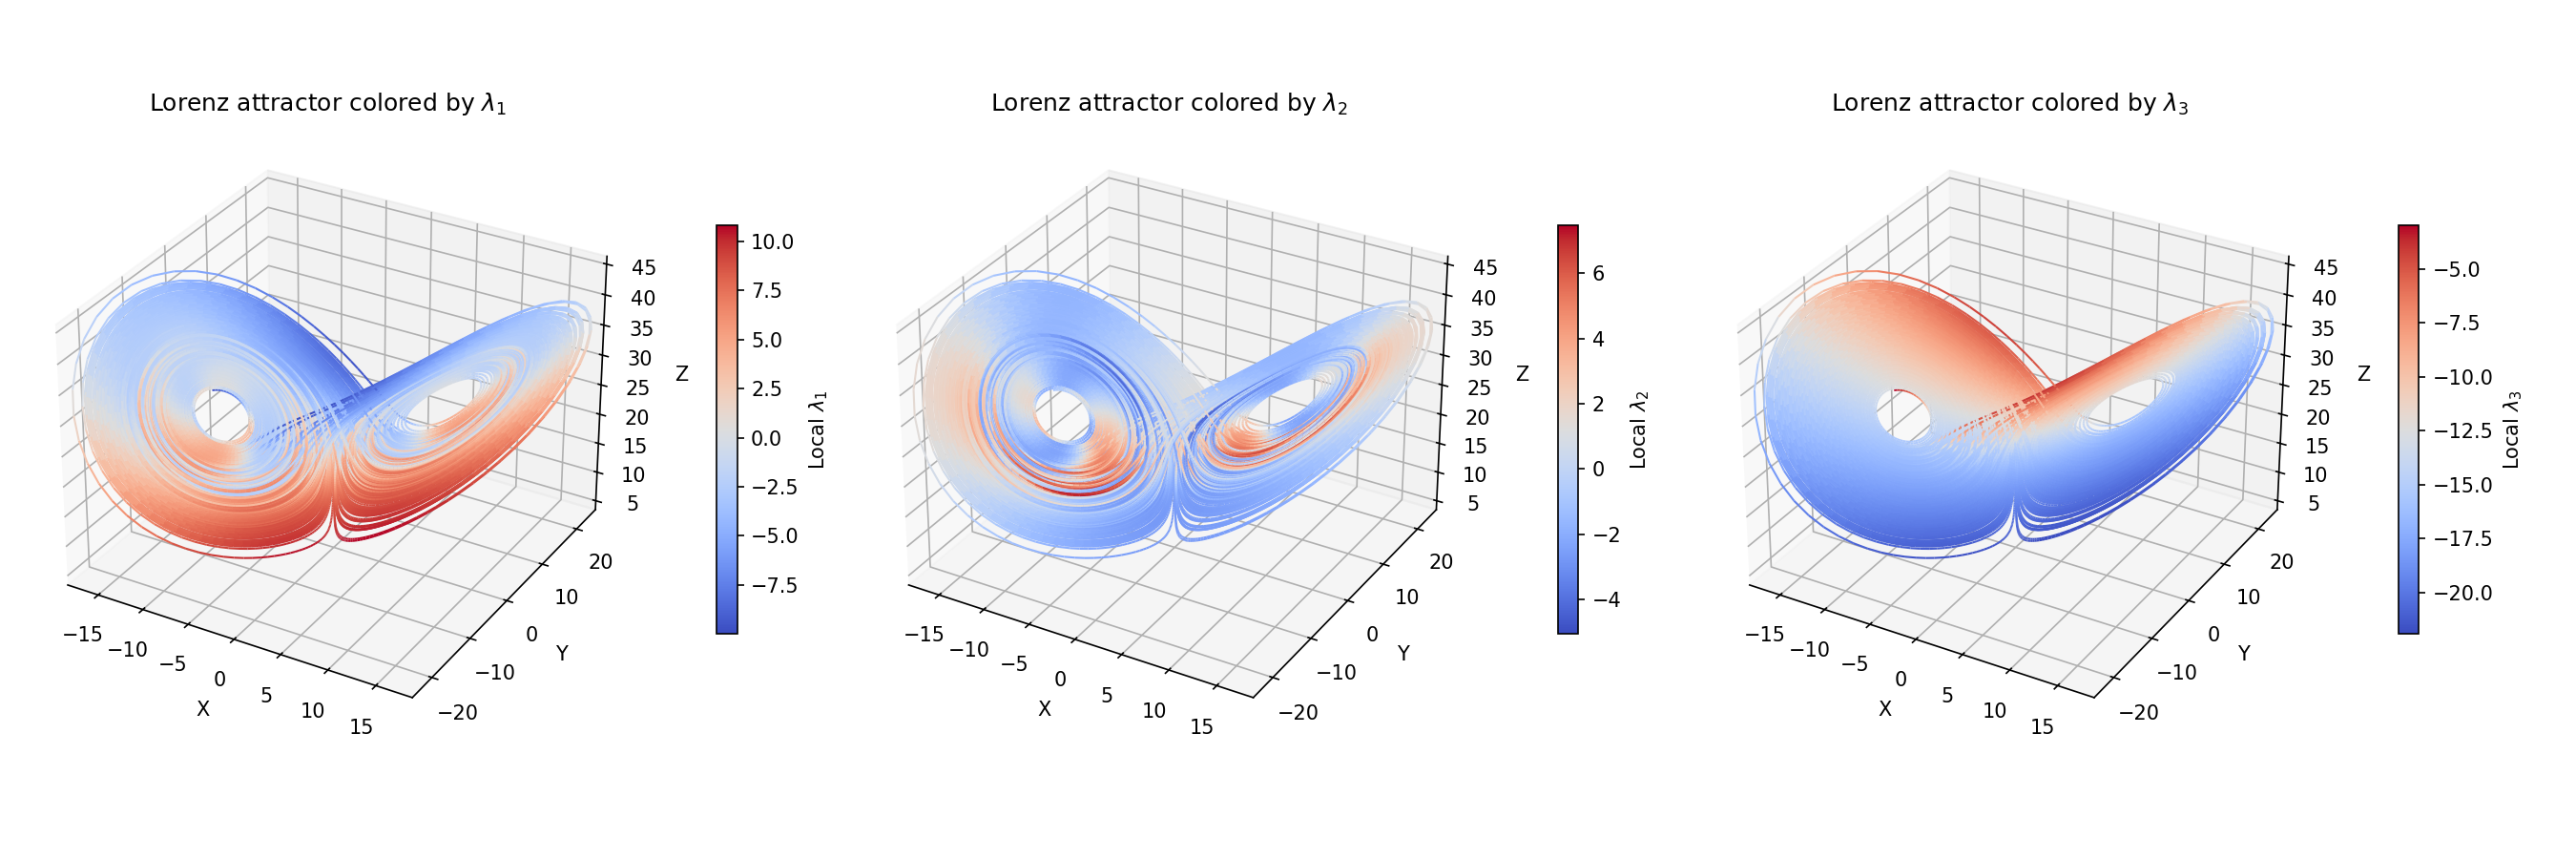
\includegraphics[width=\linewidth]{figs/lorenz_lle_heatmap.png}
    \caption{Lorenz attractor with heatmaps of the local Lyapunov exponents.}
    \label{fig:lorenz_lle_heatmap}
\end{figure}

\begin{figure}
    \centering
    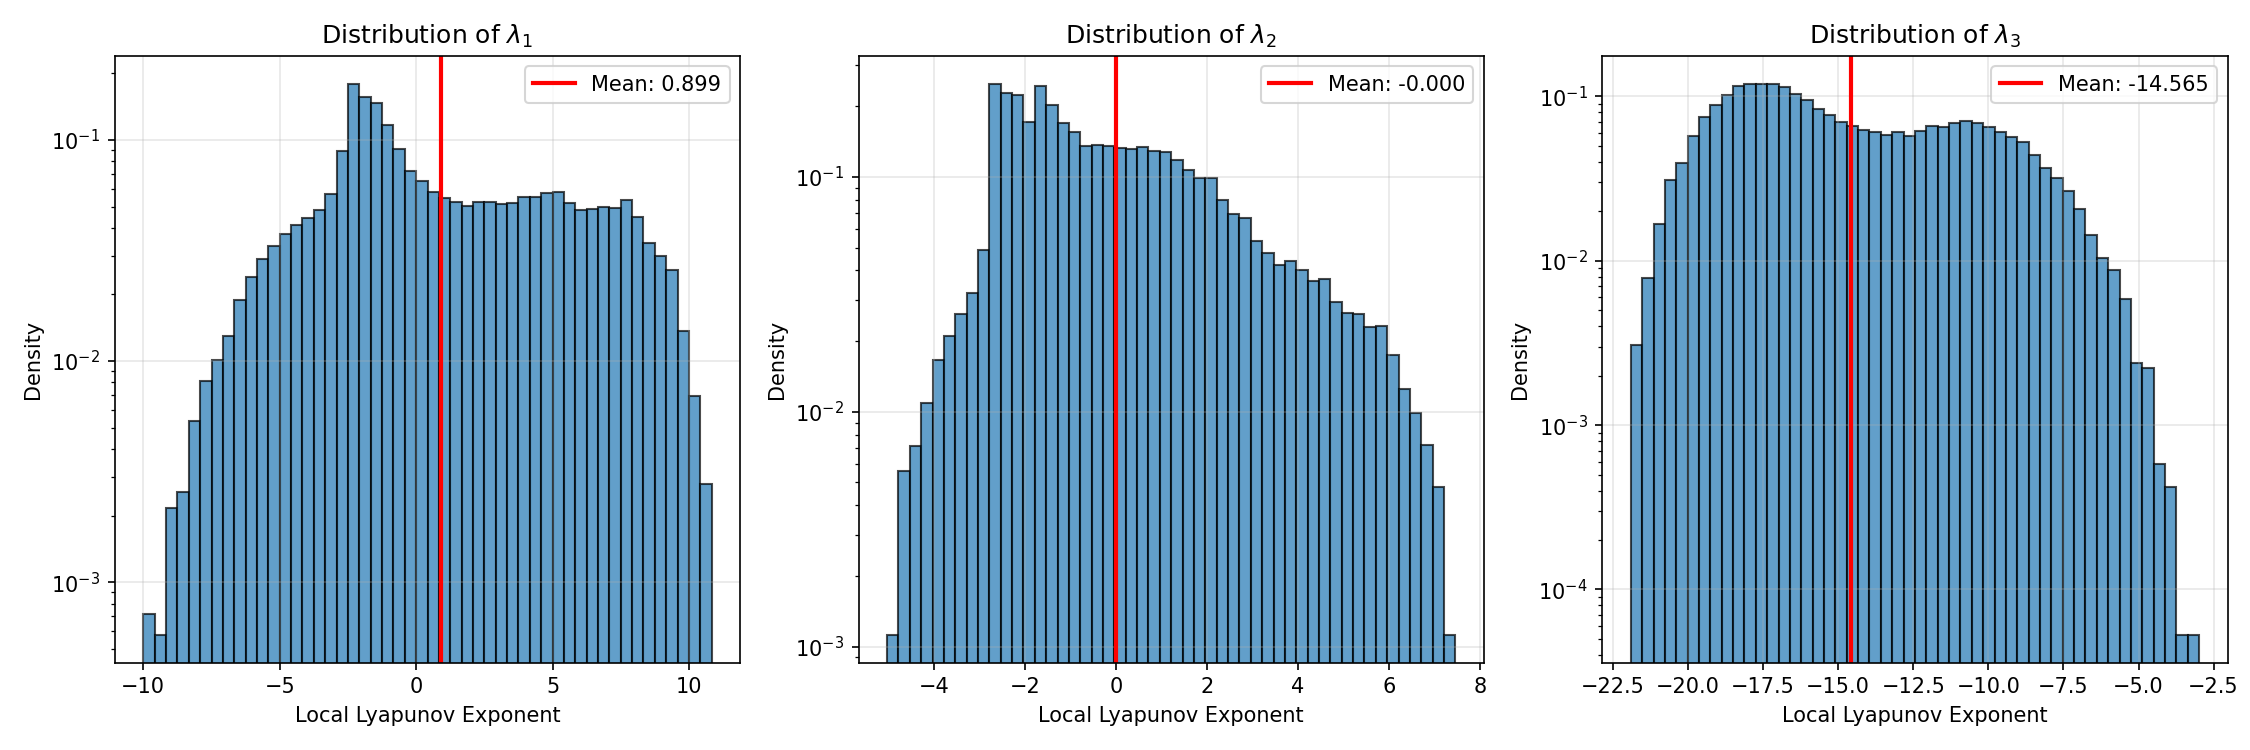
\includegraphics[width=\linewidth]{figs/lorenz_lle_histogram.png}
    \caption{Histograms of the local Lyapunov exponents along the Lorenz attractor for the standard parameters $(\sigma, \rho, \beta) = (10, 28, \frac{8}{3})$. The mean of the leading LLE distribution is close to the literature value of MLE, $\lambda_{\max} = 0.9056$ \cite{geurts_lyapunov_2020}. Obtained distributions are also consistent with those reported by \cite{ayers_supervised_2023}.}
    \label{fig:lorenz_lle_heatmap}
\end{figure}

\subsection{Neural Networks for Dynamical Systems}

In this paper, the trajectory of a chaotic dynamical system is approximated using a simple artificial neural network. Specifically, we use multi-layer perceptron (MLP) with 3 hidden layers of 10 neurons each (excluding Rössler system, where architecture was simplified to 2 layers of 5 neurons due to the low problem complexity - see [CITE ROSSLER in Methods]), residual connections, and z-score normalization. The dimensionality of the input and output layers of the neural networks was adjusted as required by the dynamical system. Fixed horizon models were trained for 20 and 200 epochs depending on the task.

The use of an MLP is motivated by the structure of the forecasting problem. The model approximates a low-dimensional one-step transition map, while the required temporal depth is introduced through repeated autoregressive application. This separation is consistent with the Serial Scaling Hypothesis: increasing the depth of the computational process is achieved through sequential rollout rather than through a wider parallel architecture \cite{liu_serial_2026}. A Transformer would not necessarily provide an advantage here, because its main strength is parallel processing of input sequences, whereas the present task requires learning a state-to-state map. The MLP therefore provides a smaller and more direct architecture for studying the effect of temporal horizon.

\subsection{Prediction Horizon as a Design Choice}

Existing work on dynamical system forecasting focuses mainly on one-step predictions. Following the existing literature on temporal horizons \cite{aceituno_temporal_2025} and as shown in later results, we argue that single-step predictions are not an optimal choice and can be replaced with longer forecasts. However, it has been shown that in chaotic systems the number of local minima in the loss landscape, called loss roughness, grows exponentially with regard to $T$ \cite{aceituno_temporal_2025}, making the problem computationally demanding.

In this paper, we set the validation horizon at $T=1$ and consistently use it as an evaluation metric. Although this choice is somewhat arbitrary, we consider it the most appropriate given the conventions in the existing literature and the need to enable meaningful benchmarking. Having decided on this, we are aware that this metric choice will not necessarily globally produce the best results. However, it is not our main objective to design a model that will achieve state-of-the-art performance on the benchmark chaotic dynamical systems; rather, given an arbitrary set of assumptions and hyperparameters or a limited amount of computational resources, we want to show the superiority of the adaptive approach over fixed-horizon models.

\subsection{Related Work}

Related approaches have demonstrated the benefits of adapting temporal decisions to the forecasting context. Pan et al. propose LeapTS, which dynamically selects the temporal scale and the advancement length used to generate different parts of a forecast \cite{pan_leapts_2026}. Their results show that learned, context-dependent scheduling can outperform both fixed and randomly generated scheduling strategies. However, LeapTS retains a predetermined total forecast horizon and adapts only the internal sequence of steps used to cover it. Similarly, varied-horizon models such as ElasTST are designed to generate forecasts for different externally specified output lengths, rather than determining which horizon is appropriate for a particular state \cite{zhang_elastst_2024}. Adaptive rollout lengths have also been studied in model-based reinforcement learning, where the rollout horizon is adjusted according to factors such as model accuracy, uncertainty, or training progress \cite{bhatia_adaptive_2022, frauenknecht_trust_2024}. These studies provide evidence that temporal horizons should not necessarily be treated as fixed hyperparameters, although their objectives and application domains differ from the supervised forecasting of chaotic systems considered here.

\subsection{Lyapunov-Based Horizon Idea} \label{lm-idea}

Depending on the dynamical system taken into account, one needs some ground truth knowledge about the system dynamics to form initial constraints and guide hyperparameter choice. In the discussed example of a Lorenz attractor, a reasonable $T_{\max}$ upon which the model could be trained is the mean lap duration, which means the averaged time the trajectory stays on one side of the attractor ($T = \text{approx. }0.7$ time unit). After that time, the behavior of the attractor cannot be predicted with reasonable accuracy by the definition of a chaotic system.

This idea can be formalized by defining the base prediction horizon as a fraction of the Lyapunov time $\frac{1}{\lambda_{\max}}$, expressed in simulation steps:

\begin{equation} \label{eq:t-base}
T_{\mathrm{base}} = \mathrm{clip}\left( \mathrm{round}\left( \frac{\gamma}{\lambda_{\max}\,\Delta t} \right),\, 1,\, T_{\max}^{\mathrm{train}} \right)
\end{equation}

Here, $\lambda_{\max}$ is the maximal Lyapunov exponent (MLE), estimated as the mean local Lyapunov exponent along the training trajectory, $\Delta t$ is the simulation time step, $T_{\max}^{\mathrm{train}}$ is the largest horizon used in training, and $\gamma$, called the \emph{Lyapunov fraction}, is an empirically chosen parameter: the fraction of the Lyapunov time up to which predictions remain reliable. If $\lambda_{\max} \le 0$, we set $T_{\mathrm{base}} = T_{\max}^{\mathrm{train}}$.

In addition to the MLE-informed base horizon, we extended this idea to include the local divergence rate in rollout lengths. Instead of applying a globally fixed $T$ to every point of the trajectory, the proposed approach assigns a state-dependent horizon:

\begin{equation}
T_t = \pi(\mathbf{x}_t),
\end{equation}

Here, $\mathbf{x}_t$ denotes the current system state and $\pi$ represents a predefined or learned horizon-selection rule. The underlying hypothesis is that the appropriate prediction horizon depends on the local predictability of the dynamics.

We used FTLEs as indicators of the rate at which the nearby trajectories diverge throughout the manifold. A positive and large FTLE indicates reduced predictability and motivates a shorter rollout, whereas a smaller or negative exponent suggests that longer predictions may remain informative. Conceptually, the selection rule is therefore expected to satisfy

\begin{equation}
\text{FTLE}(\mathbf{x}_t) \uparrow
\quad \Longrightarrow \quad
T_t \downarrow.
\end{equation}

The sample-wise horizons are centered around $T_{\mathrm{base}}$ and vary depending on their FTLEs within a given range. For example, in the basic approach we set the spread parameter $v$ to 1, so that the horizons are distributed between $T_{\mathrm{base}} \pm 1$.

The adaptive approach aims to combine the optimization stability of short-horizon training with the long-term benefits of longer rollouts by assigning each training sample a horizon suited to its local dynamical properties. Its effectiveness is evaluated against the fixed horizon and a randomized FTLE $\rightarrow$ horizon mapping. The latter is particularly important, as it distinguishes the benefit of meaningful state-dependent adaptation from the regularizing effect of merely exposing the model to multiple rollout lengths.

\newpage

\section{Methods}

\subsection{Fixed Horizon Baseline} \label{fixed_horizon}

Initially, we train a set of neural networks to approximate the dynamical systems described above using standard parameters (see \ref{dynamical_systems}). During simulation, we used a burn-in period to discard the initial $\lceil \frac{10.0}{\Delta t} \rceil$ steps before the trajectory was properly set on the attractor.

The training set consists of 100 trajectories and the validation set of 20 trajectories, 1000 steps per each trajectory. We tested with time steps $\Delta t=0.05, 0.08, 0.1$ and roll-out the simulation up to $T_{\max}=10$ steps in the future, summing up to physical times $\tau = 0.50, 0.80, 1.0$, respectively.

In order to reproduce Fig. 5 from \cite{aceituno_temporal_2025}, we trained 20 MLPs with fixed seeds: (1) for 20 epochs and (2) for 200 epochs; with each training horizon $T \in \{1, 2, ..., 10\}$ and validated them at the same horizon values $T_{\text{val}}$ (see Fig. \ref{fig:mse_fixed}). Note that at this stage the results already differ slightly from the original paper, as we were able to retrieve the Lorenz trajectories with reasonable loss values up to a temporal horizon of $\tau = 0.1$. The Mean Squared Error (MSE) obtained for each $T_{\text{val}}$ is used as an evaluation metric.

Based on cross-validation performance, we report two horizon values for which the median MSE was minimal: (1) across all $T_{\mathrm{val}}$, and (2) when validated only on $T_{\mathrm{val}} = 1$. From now on, this is our baseline for comparison with the adaptive horizon models.

\begin{figure}
    \centering
    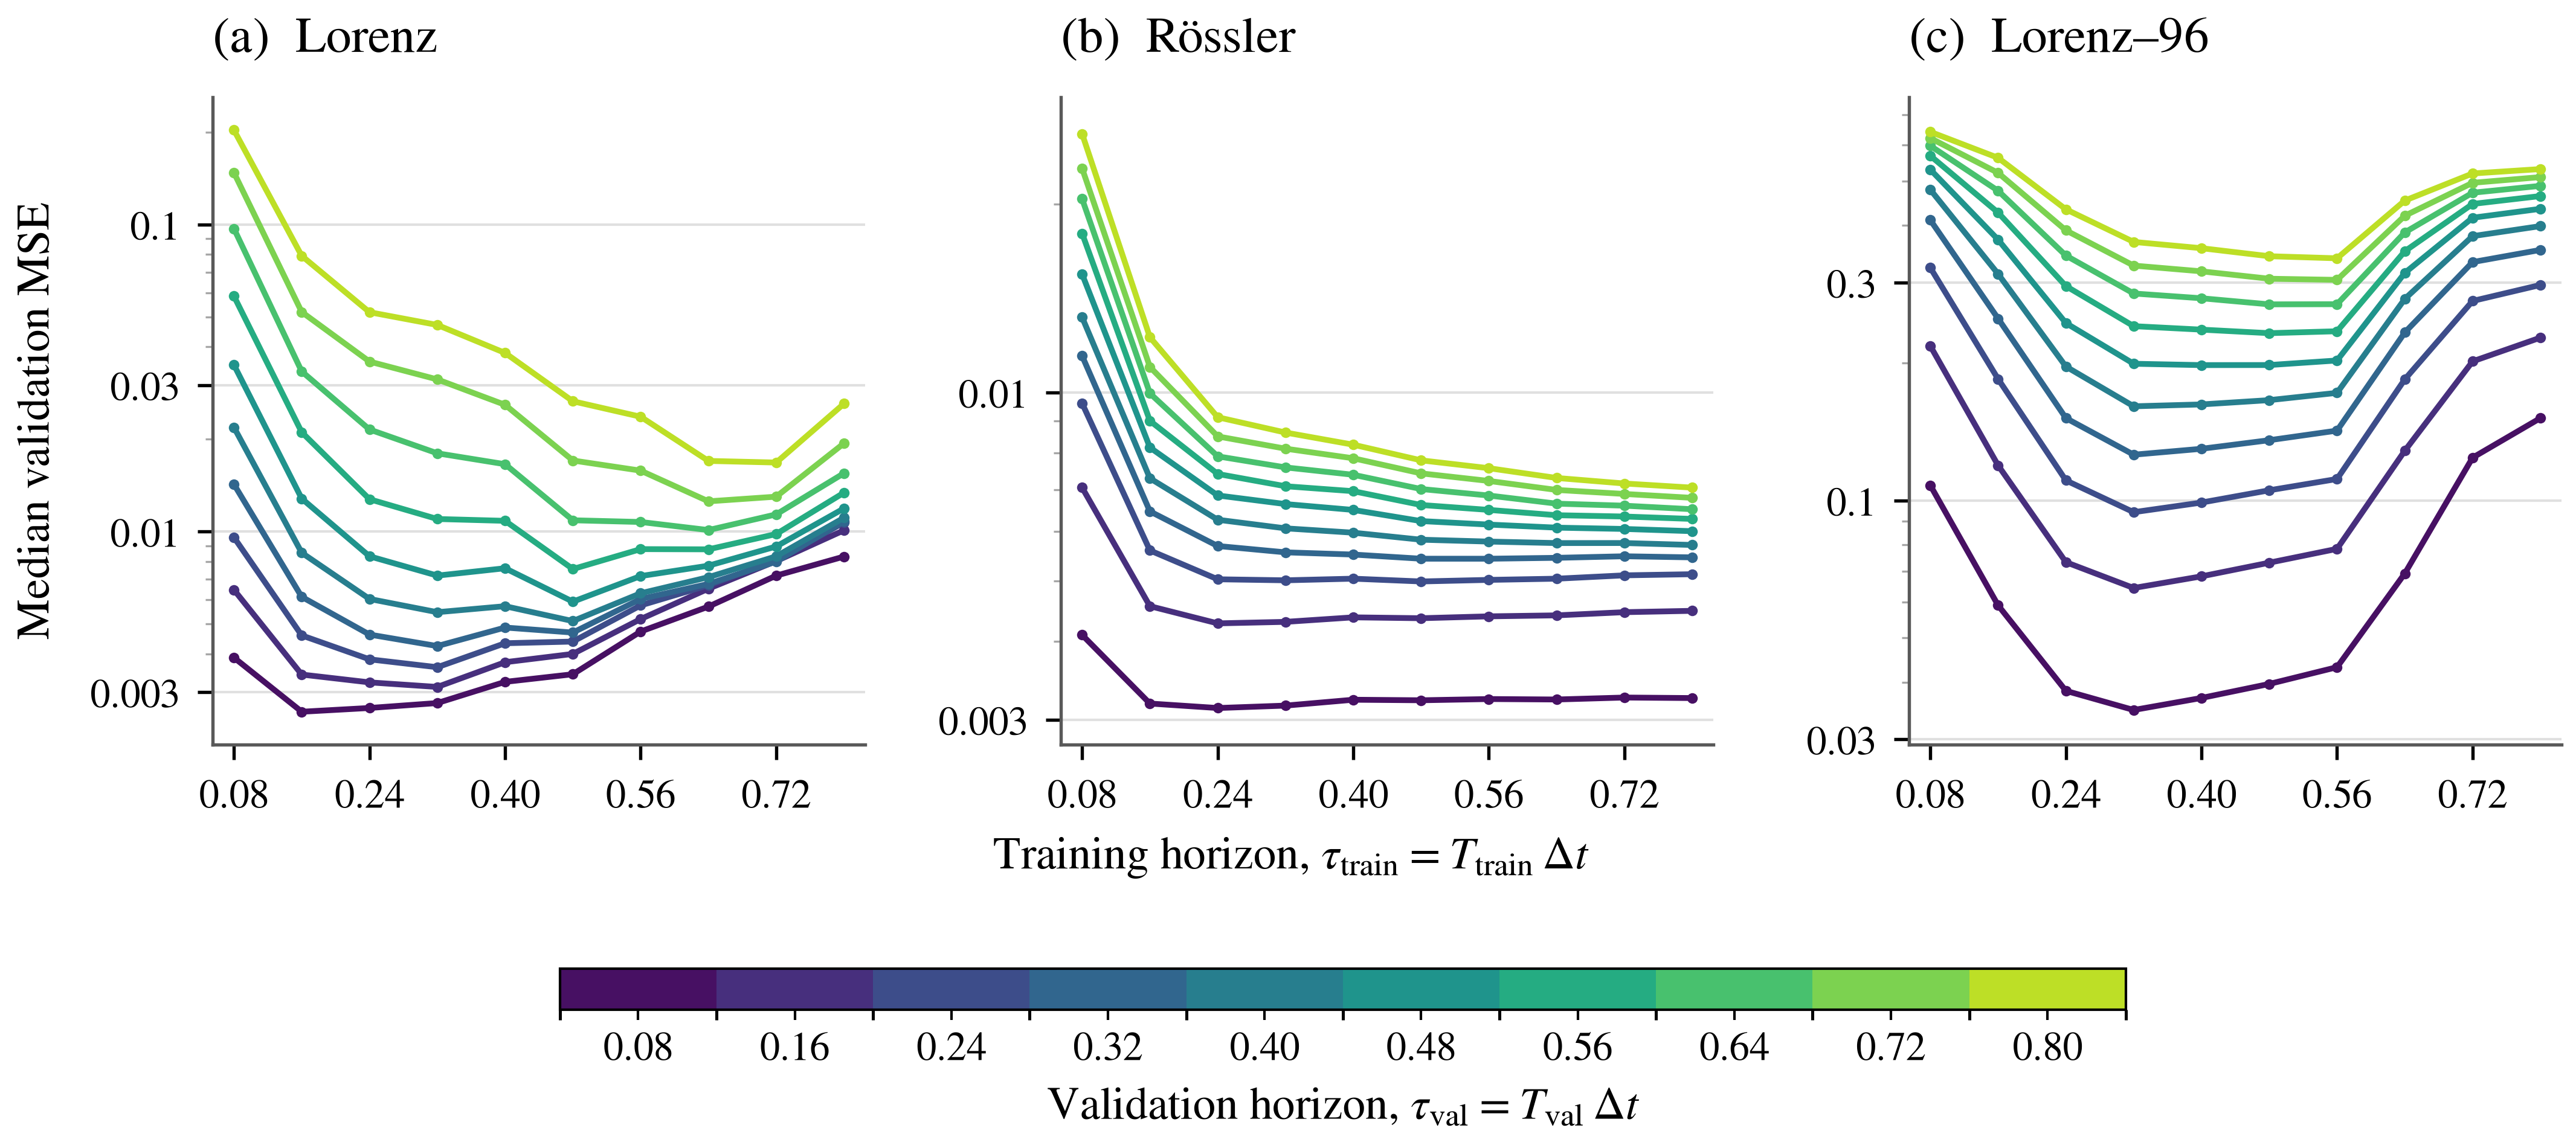
\includegraphics[width=\linewidth]{figs/mse_dt_08_fixed_200.png}
    \caption{\textbf{Exemplary cross-validation curves of the fixed horizon MLPs trained with $\mathbf{\Delta t = 0.08}$ for 200 epochs.} Temporal horizons used during training are shown on the x-axis and average of the minimum validation MSE across all $T_{\mathrm{val}}$ on the y-axis. Each line represents different validation horizon.}
    \label{fig:mse_fixed}
\end{figure}

\subsection{Budget-Based Approach}

Although adapting the horizon based on the uncertainty of the system is conceptually valid, our initial experiments show that it does not yield satisfactory results compared to fixed horizon baseline. Calculating FTLEs for every point on the trajectory is also computationally demanding. Therefore, we define the objective as \emph{the computation budget-based horizon search}.

We argue that to find the optimal performance-learnability tradeoff described in \cite{aceituno_temporal_2025} one does not need to train a number of fixed horizon models and perform a grid search with regard to the prediction horizon, but one could use the same amount of computational resources to train one model with an adaptive technique instead to obtain a better fit. In the following section, we discuss various approaches to this task.

\subsubsection{Linear Horizon Scheduler}

First, we try a naive approach to finding the optimal horizon by setting up a \textbf{linear horizon scheduler (LS)}, where every 20 epochs $T$ is increased by one. Similarly to the fixed setup, we trained 20 adaptive models for each system and $\Delta t$ up to $T_{\max}$ for 200 epochs and compared them against fixed models trained for 20 epochs. In this way, the same amount of resources was used in the fixed and adaptive setting (10 x 20 epochs vs. 200 epochs).

In this case, as expected from \cite{aceituno_temporal_2025}, the validation loss explodes in adaptive models, since the choice of $T_{\max} = 10$ is very arbitrary and does not reflect the system's uncertainty in any way. As can be observed in Fig. \ref{fig:mse_fixed}, system's predictability depends directly on the Lyapunov time; for example, in Lorenz and Lorenz-96 , $\tau = 0.80$ is already too long a rollout, so training with this horizon causes the loss to explode. Meanwhile, the Rössler system can be effectively trained with $\tau = 0.80$, making linear scheduler models perform considerably well.

\subsubsection{Cross-Validation Minimum Search}

For the aforementioned reasons, the conclusion was drawn that the $T$ increase must be forced to some extent, but stopped when the validation loss explodes, ideally at the "minimum" of the cross-validation curve (see Fig. \ref{fig:mse_fixed}). Increasing the training horizon can improve rollout prediction, but can also make optimization harder. Stopping immediately when validation performance deteriorates may favor short horizons, since the model needs time to adapt. One needs to find a trade-off between improving general learnability on the one hand and preventing an explosion of gradients on the other (see \cite{aceituno_temporal_2025}).

Therefore, we decided to introduce the \textbf{cross-validation-based approach (CV)} with the following logic. Training starts at a horizon of one, and after each epoch, the model is evaluated using MSE averaged over a fixed ten-step rollout. This score is smoothed over three epochs. Each horizon is trained for at least five and at most twenty epochs. After the minimum duration, three consecutive checks without an improvement exceeding 1\% trigger a horizon increase. At each stage boundary, the current parameters and the smoothed score are cached. The horizon increases by one until the configured maximum is reached; training then continues at that maximum until the training budget is exhausted.

After training, the method selects the largest horizon whose cached score is within 5\% of the best observed score. Among eligible checkpoints at the same horizon, it selects the lowest-scoring one and restores its parameters. Validation deterioration does not directly stop training.

This approach is still not ideal, as it is hard to distinguish whether the validation loss improvement stems from finding a better horizon fit or simply from more training time. Therefore, the CV method \emph{is not identical and cannot be confused} with formerly presented cross-validation that we performed after training (see \ref{fixed_horizon}).

\subsubsection{Lyapunov-Mean Horizon}

To incorporate the information about local system instability into the training, we introduce the idea of a \textbf{Lyapunov-Mean horizon (LM)}. In this setting, each training sample is assigned its own prediction horizon, drawn from a narrow range centered on a base horizon $T_{\mathrm{base}}$ with a fixed spread $v$ (see \ref{lm-idea}).

Each sample is assigned a horizon from a narrow range around the base horizon $T_{\mathrm{base}}$ defined in Eq.~\eqref{eq:t-base}:

$$T_{\min} = \max(1,\, T_{\mathrm{base}} - v), \qquad T_{\max} = \min(T_{\mathrm{base}} + v,\, T_{\max}^{\mathrm{train}}),$$

With spread $v = 1$ (see \ref{lm-idea}).

\paragraph{FTLE-based assignment.} For every state $x_m$ of the training trajectory, we compute the largest forward finite-time Lyapunov exponent over a window of $T_{\mathrm{base}}$ steps:

$$\lambda_m = \mathrm{FTLE}_{T_{\mathrm{base}}}(x_m), \quad m = 0, \dots, N - T_{\mathrm{base}} - 1,$$

where $N$ is the length of the training trajectory. The FTLEs are standardized over the trajectory:

$$z_m = \frac{\lambda_m - \mu_{\lambda}}{\sigma_{\lambda}},$$

Where $\mu_{\lambda}$ and $\sigma_{\lambda}$ are the mean and standard deviation of the FTLEs. The standardized scores are scaled by the half-width of the horizon range,

$$r = \max\left( 1, \frac{T_{\max} - T_{\min}}{2} \right),$$

and the horizon of sample $m$ becomes

$$T_m = \mathrm{clip}\left( \mathrm{round}(T_{\mathrm{base}} - z_m r),\, T_{\min},\, T_{\max} \right).$$

Interpretation:
\begin{itemize}
    \item If $\lambda_m > \mu_{\lambda}$, then $z_m > 0$ and $T_m$ becomes shorter: locally more chaotic states are trained on shorter rollouts.
    \item If $\lambda_m < \mu_{\lambda}$, then $z_m < 0$ and $T_m$ becomes longer: locally more predictable states are trained on longer rollouts.
\end{itemize}

\textbf{Note}: Because normalization uses statistics of the training trajectory, the horizons reflect relative instability within that trajectory, not the absolute magnitude of the FTLE.

\paragraph{Training budget.} LM models were compared with fixed-horizon models under a matched training budget. Computing FTLEs is expensive, so instead of a fixed number of epochs, LM training stops once it reaches the total number of operations used for training the corresponding sweep of fixed models, $T \in \{1, \dots, T_{\max}^{\mathrm{train}}\}$. For example, if training one set of fixed models for $T \in \{1, \dots, 10\}$ took 10000 steps in total, each LM model was also given a budget of 10000 steps including FTLE computation.

\subsubsection{Randomized Lyapunov-Mean Horizon}

The LM models differ from fixed-horizon training in two ways: they expose the model to a range of rollout lengths, and they tie each rollout length to the local predictability of the sample's initial state. To separate the effect of horizon diversity alone from the effect of using information about local divergence, we train an additional set of randomized Lyapunov-mean (LMR) models as an ablation. LMR models are constructed exactly as LM models: they
use the same base horizon $T_{\mathrm{base}}$, the same admissible range $[T_{\min}, T_{\max}]$, and the same FTLE-based mapping, which produces a horizon $T_n$ for every training sample $n = 1, \dots, N$. The horizons are then randomly permuted across samples before training:

\begin{equation}
  \tilde{T}_n = T_{\pi(n)}, \qquad \pi \sim \mathcal{U}(S_N),
  \label{eq:lmr_permutation}
\end{equation}

Where $S_N$ denotes the set of permutations of $\{1, \dots, N\}$. The permutation $\pi$ is drawn once with a fixed seed and kept constant throughout training. Because a permutation preserves the multiset $\{T_n\}_{n=1}^{N}$, LMR models see exactly the same distribution of horizons as LM models, with the same mean, variance and range, and therefore the same number of rollout steps per epoch. The only property removed is the correspondence between a sample's FTLE $\Lambda_T(\mathbf{x}_n)$ and its assigned horizon. Consequently, if LM models outperform LMR models, the improvement can be attributed to the FTLE-informed assignment of horizons. If the two perform comparably, the benefit of LM comes mainly from training on a mixture of rollout lengths.

\newpage

\section{Results (work in progress...)}

We ran a set of experiments on each dynamical system:

\begin{itemize}
    \item Fixed models trained for 20 epochs (for budget-based comparison),
    \item Fixed models trained for 200 epochs (for comparison with no computation constraint),
    \item Linear Scheduler models trained for 200 epochs,
    \item Budget-based Lyapunov-Mean models trained with a constraint on computational resources set on the summarized number of steps used to train all 20-epochs fixed models (usually training stopped around epoch 150),
    \item Lyapunov-Mean models trained for 200 epochs,
    \item Randomized Lyapunov-Mean models trained for 200 epochs.
\end{itemize}

The models were cross-validated on the same set of horizon values $T_{{\text{val}}} \in \{1, \dots,10\}$ that was used for training. For each seed and $T_{\text{val}}$, the error is the MSE averaged over the first $T_{\text{val}}$ steps of an autoregressive rollout. As a performance measure we report (1) the median of the one-step MSE across 20 seeds ($T_{\text{val}} = 1$) and (2) the median over all 20 seeds × 10 values of $T_{\text{val}}$. Each yields a single value per method, enabling a straightforward comparison.

\subsection{General Observations}

Comparing the 

\subsection{Lorenz System}

The table below (see Tab. \ref{tab:lorenz_mse_results}) shows the comparison of the training session for the Lorenz attractor where $T_{\max} = 10$, which means that:

\begin{itemize}
    \item Fixed models were trained for $T \in \{1, 2, ..., 10\}$ for 20 epochs each,
    \item Linear Scheduler models were trained for 200 epochs until $T_{\max} = 10$,
    \item Linear Scheduler models with ES were usually trained for 100-120 epochs until ES conditions were met,
    \item Cross-Validation-Based models were usually trained for 100-120 epochs until the online validation conditions were met,
    \item Lyapunov-Based models used the mean summed time used to train all fixed models until $T=10$.
\end{itemize}

\begin{table}[h]
\centering
\begin{tabular}{cccc}
\toprule
\makecell{Method} & \makecell{MSE $\pm$ 95\% CI} \\
\midrule
Fixed $T=3$ & 0.003857 $\pm$ 0.000398 \\
Linear Scheduler & 0.004153 $\pm$ 0.000286 \\
Linear Scheduler with ES & 0.003605 $\pm$ 0.000281 \\
Lyapunov-Based ($\sigma=5$) & 0.003318 $\pm$ 0.000469 \\
Lyapunov-Based ($\sigma=3$) & 0.003668 $\pm$ 0.000248 \\
Cross-Validation-Based & \textbf{0.003295 $\pm$ 0.000341} \\
\bottomrule
\end{tabular}
\caption{Lorenz: Median MSE at $T_{\text{val}}=1$ over 20 seeds, with 95\% confidence intervals.}
\label{tab:lorenz_mse_results}
\end{table}

Cross-Validation-Based models yield the best results across all considered methods, showing consistent improvements over the fixed baseline across all budgets from $T_{\max} = 3$ onward. This result suggests that part of the benefit may come not only from adapting the horizon itself, but also from avoiding excessive training at large horizons once validation performance stops improving. Early stopping therefore acts as a stabilizing mechanism, preventing the model from entering training regimes where the forecasting target becomes too difficult or noisy.

The Lyapunov-Based method with $\sigma=5$ is a close second and performs better than the corresponding variant with $\sigma=3$. In the budget comparison for $\sigma=5$, the best fixed-horizon baseline has a lower marginal median MSE for
$T_{\max} \in \{1, 2, ..., 7\}$, while the Adaptive Horizon model has a lower marginal median for $T_{\max} \in \{8, 9, 10\}$. Effectively, the advantage of the adaptive horizontal model appears only once the available training budget becomes sufficiently large. In low-budget settings, the additional variability introduced by adaptive horizons may instead make the optimization problem harder. Additionally, training time constraints keep the number of epochs that models are trained on low, as a lot of computational resources is used for LLE calculation. This suggests that adaptive horizon training may require enough exposure to longer rollout regimes before its benefits become visible.

Tables \ref{tab:budget_comparison_cv} and \ref{tab:budget_comparison_ah5} present a detailed comparison of the two best methods. The difference $\Delta = \text{MSE}_{\text{fixed}} - \text{MSE}_{\text{adaptive}}$ is visualized in Figures \ref{fig:budget_deltas_cv} and \ref{fig:budget_deltas_ah5}.

\begin{table}[ht]
\centering
\small
\resizebox{\textwidth}{!}{%
\begin{tabular}{cccccc}
\toprule
$T_{\max}$ &
\makecell{Best \\ fixed $T$} &
\makecell{Fixed MSE} &
\makecell{Adaptive MSE} &
$\Delta$ &
\makecell{Adaptive \\ win rate} \\
\midrule
  2  & 2 & $\mathbf{0.003946 \pm 0.000376}$ & $0.004673 \pm 0.000587$ & $-0.000173$ & 40\% \\
  3  & 3 & $\mathbf{0.003857 \pm 0.000398}$ & $0.003923 \pm 0.000436$ & $+0.000206$ & 65\% \\
  4  & 3 & $0.003857 \pm 0.000398$ & $\mathbf{0.003410 \pm 0.000403}$ & $+0.000480$ & 75\% \\
  5  & 3 & $0.003857 \pm 0.000398$ & $\mathbf{0.003644 \pm 0.000386}$ & $+0.000565$ & 65\% \\
  6  & 3 & $0.003857 \pm 0.000398$ & $\mathbf{0.003401 \pm 0.000348}$ & $+0.000748$ & 65\% \\
  7  & 3 & $0.003857 \pm 0.000398$ & $\mathbf{0.003797 \pm 0.000358}$ & $+0.000572$ & 65\% \\
  8  & 3 & $0.003857 \pm 0.000398$ & $\mathbf{0.003576 \pm 0.000341}$ & $+0.000505$ & 70\% \\
  9  & 3 & $0.003857 \pm 0.000398$ & $\mathbf{0.003386 \pm 0.000349}$ & $+0.000643$ & 85\% \\
  10 & 3 & $0.003857 \pm 0.000398$ & $\mathbf{0.003295 \pm 0.000341}$ & $+0.000665$ & 80\% \\
\bottomrule
\end{tabular}%
}
\caption{Budget-based comparison for $T_{\text{val}} = 1$ between the Cross-Validation-Based method and the best fixed-horizon baseline available under each budget. Each MSE is the median over 20 seeds with a 95\% confidence interval. The reported $\Delta$ is the median of the 20 paired per-seed differences $\text{MSE}_{\text{fixed}}-\text{MSE}_{\text{CV-based}}$. Positive $\Delta$ favors the Cross-Validation Based method. The $T_{\max}=1$ case is omitted because the adaptive and fixed models are equivalent.}
\label{tab:budget_comparison_cv}
\end{table}

\begin{table}[ht]
\centering
\small
\resizebox{\textwidth}{!}{%
\begin{tabular}{cccccc}
\toprule
$T_{\max}$ &
\makecell{Best \\ fixed $T$} &
\makecell{Fixed MSE} &
\makecell{Adaptive MSE} &
$\Delta$ &
\makecell{Adaptive \\ win rate} \\
\midrule
  1  & 1 & $\mathbf{0.005573 \pm 0.000844}$ & $0.007994 \pm 0.003158$ & $-0.000935$ & 45\% \\
  2  & 2 & $\mathbf{0.003946 \pm 0.000376}$ & $0.005904 \pm 0.001316$ & $-0.001588$ & 15\% \\
  3  & 3 & $\mathbf{0.003857 \pm 0.000398}$ & $0.005178 \pm 0.000396$ & $-0.001049$ & 10\% \\
  4  & 3 & $\mathbf{0.003857 \pm 0.000398}$ & $0.004675 \pm 0.000432$ & $-0.000379$ & 25\% \\
  5  & 3 & $\mathbf{0.003857 \pm 0.000398}$ & $0.004151 \pm 0.000444$ & $-0.000254$ & 35\% \\
  6  & 3 & $\mathbf{0.003857 \pm 0.000398}$ & $0.003878 \pm 0.000452$ & $+0.000031$ & 50\% \\
  7  & 3 & $\mathbf{0.003857 \pm 0.000398}$ & $0.003865 \pm 0.000479$ & $+0.000091$ & 55\% \\
  8  & 3 & $0.003857 \pm 0.000398$ & $\mathbf{0.003709 \pm 0.000515}$ & $+0.000106$ & 75\% \\
  9  & 3 & $0.003857 \pm 0.000398$ & $\mathbf{0.003406 \pm 0.000533}$ & $+0.000428$ & 75\% \\
  10 & 3 & $0.003857 \pm 0.000398$ & $\mathbf{0.003318 \pm 0.000469}$ & $+0.000536$ & 75\% \\
\bottomrule
\end{tabular}%
}
\caption{Budget-based comparison for $T_{\text{val}} = 1$ between the Lyapunov-Based with $\sigma=5$ models and the best fixed-horizon baseline available under each budget. Each MSE is the median over 20 seeds with 95\% confidence intervals. The reported $\Delta$ is the median of the 20 paired per-seed differences $\text{MSE}_{\text{fixed}}-\text{MSE}_{\text{adaptive}}$. Positive
$\Delta$ favors the adaptive model.}
\label{tab:budget_comparison_ah5}
\end{table}

\begin{figure}
    \centering
    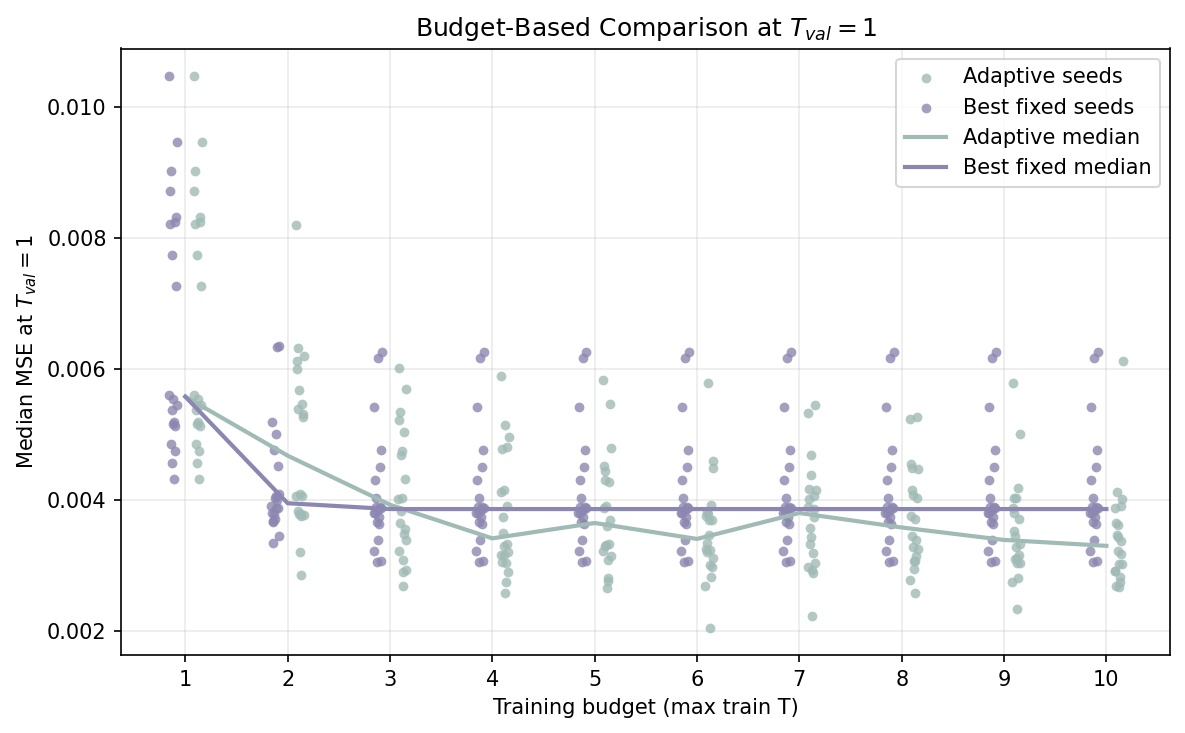
\includegraphics[width=\linewidth]{figs/budget_comparison_cv.png}
    \caption{Budget-based comparison of the best fixed ($T = 3$) and Cross-Validation Based models.}
    \label{fig:budget_deltas_cv}
\end{figure}

\begin{figure}
    \centering
    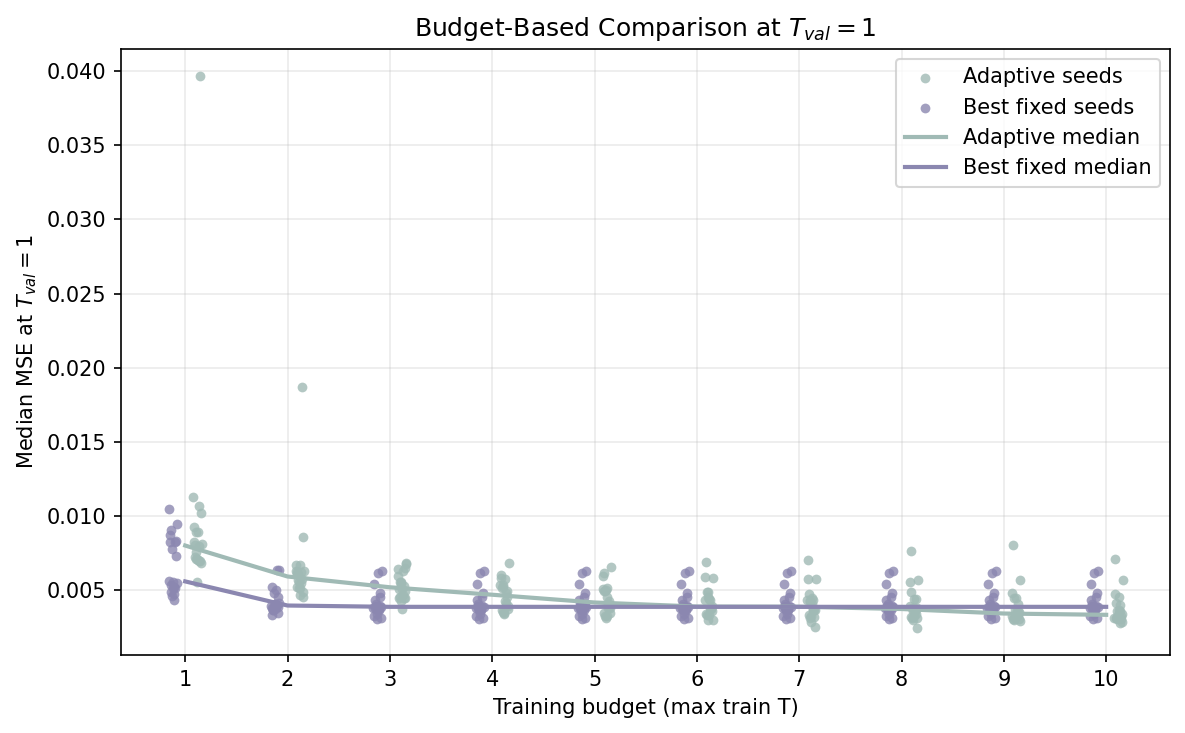
\includegraphics[width=\linewidth]{figs/budget_comparison_ah5.png}
    \caption{Budget-based comparison of the best fixed ($T = 3$) and Adaptive Horizon models centered around $\sigma = 5$. Function flattens for fixed model because model trained with $T = 3$ outperforms models with larger $T$ values and it is therefore selected as the best.}
    \label{fig:budget_deltas_ah5}
\end{figure}

The budget-based results show that the relative performance of the adaptive and fixed-horizon methods depends on both the training method and the available computational budget. The Adaptive Horizon method requires a sufficiently large budget before outperforming the best fixed-horizon baseline, whereas the Linear Scheduler with ES achieves a lower marginal median MSE for every budget
considered below. Please note that in the case of ES, adaptive training uses less resources than equivalent fixed models.

The results suggest that exposing the model to multiple training
horizons can improve single-step forecast performance when the training
budget is controlled. At $T_{\text{val}}=1$, the best fixed-horizon
baseline, trained with $T=3$, achieves a median MSE of 0.003857. The
Linear Scheduler with Early Stopping reduces this value to 0.003605.
The lowest observed median among the verified 20-seed methods is
obtained by the Cross-Validation Based method, with an MSE of 0.003295,
followed closely by the Adaptive Horizon method with $\sigma=5$, with
an MSE of 0.003318. These results indicate that adapting the training
horizon or the stopping point can provide a more effective training
signal than selecting a single fixed horizon when performance is
evaluated at $T_{\text{val}}=1$.

\subsection{Rossler System}

The models were trained with the same objective as Lorenz.

\begin{table}[h]
\centering
\begin{tabular}{cc}
\toprule
\makecell{Method} & \makecell{MSE $\pm$ 95\% CI} \\
\midrule
Fixed $T=3$ & \textbf{0.003831 $\pm$ 0.000120} \\
Linear Scheduler & 0.003995 $\pm$ 0.004150 \\
Linear Scheduler with ES & 0.003973 $\pm$ 0.004156 \\
Lyapunov-Based ($\sigma=5$) & 0.004148 $\pm$ 0.000032 \\
Cross-Validation-Based & 0.003911 $\pm$ 0.000297 \\
\bottomrule
\end{tabular}
\caption{Rossler: Median MSE at $T_{\mathrm{val}}=1$ over 20 seeds, with 95\% confidence intervals.}
\label{tab:rossler_mse_results}
\end{table}

\clearpage
\bibliographystyle{plain}
\bibliography{references}

\clearpage
\appendix

\section{Methods Description}
\label{app:method-description}

\subsection{Weighted Loss with Finite-Time Lyapunov Exponents}
\label{app:weighted-loss}

To further improve the performance of the system by measuring how nearby trajectories diverge at a certain point on the trajectory, we introduced the idea of soft-weighted loss over a fixed roll-out horizon. We used the best horizon value $T = 5$ obtained from previous experiments.

For each state starting at state $x_i$, the model rolls forward auto-regressively until a fixed number of $T$ steps, and the Finite-Time Lyapunov Exponent score $\lambda_i$ is calculated, measuring a short-window maximum local expansion:

$$\lambda_i = \frac{1}{W \cdot dt} \cdot \ln \sigma_{\text{max}}(M_i)$$

Where:
\begin{itemize}
    \item $W$ is the window size,
    \item $M_i$ is the tangent map over the next $W$ steps,
    \item $\sigma_{\text{max}}(M_i)$ is the largest singular value.
\end{itemize}

For each roll-out step, a predictability budget is computed, approximating how many Lyapunov times have elapsed by step $j$:

$$s_{i, j} = \text{max}(\lambda_i, 0) \cdot j \cdot dt$$

Then, soft weights are assigned:

$$a_{i, j} = \text{max} \left ( \text{sigmoid} \left ( \frac{\rho  - s_{i, j}}{\theta} \right ), w_{\text{min}} \right )$$

With default parameter values:
\begin{itemize}
    \item $\rho = 1.0$: Predictability budget threshold. A larger $\rho$ means high weight for longer roll-out steps even for unstable states.
    \item $\theta = 0.25$: Temperature (softness of the cutoff). Small temperature makes the transition sharp, large temperature makes the weight decay gradually.
    \item $w_{\text{min}} = 0.05$: Minimum unnormalized weight. Prevents the long-horizon errors from vanishing.
\end{itemize}

The loss is calculated as follows:

$$L_i = \alpha \cdot \text{MSE} (\hat{x}_{i+1} \text{, } x_{i+1}) + (1 - \alpha) \cdot \sum_{\tau = 1}^{\tau_{\text{max}}} w_{i+\tau} \text{MSE}(\hat{x}_{i+\tau} \text{, } x_{i+\tau})$$

Where $\alpha$ is the strength of the one-step anchor. A larger $\alpha$ prioritizes accurate local dynamics.

\end{document}
